\documentclass{book}

\usepackage[b6paper]{geometry}
\usepackage{graphicx}

% Page numbers
\usepackage{pgfornament}
\usepackage{fancyhdr}
\fancyhf{}
\fancyfoot[C]{
  \pgfornament[anchor=south,width=5mm]{11}\ \thepage\ \pgfornament[anchor=south,width=5mm]{14}
}
\pagestyle{fancy}
%\fancypagestyle{plain}{}
%\fancypagestyle{empty}{}

%% Chapters should use empty style instead of plain style
\makeatletter
\let\ps@plain\ps@empty
\makeatother

%% Titles
\usepackage{titlesec}
\titleformat{\chapter}[display]
  {\normalfont\chapfnt\bfseries}{}{0pt}{\chapfnt}

%% Encodings
\usepackage{polyglossia}
\setmainlanguage{hungarian}
\usepackage{xepersian}

%% Fonts
\setmainfont{fbb}
\newfontfamily\poemfont{IranNastaliq:style=Regular}
\newfontfamily\persianfont[Script=Arabic]{Amiri}

%% Verse environment
\usepackage{varwidth}
\newenvironment{Verse}
  {\center\varwidth{\linewidth}}
  {\endvarwidth\endcenter} 

%% poem command
\newcommand{\poemnotoc}[6] {
\begin{center}#1\smallskip{\RTL\persianfont #2}\end{center}
\vspace{1cm}
{\RTL\large\poemfont\begin{tabular}{r r}#3\end{tabular}}
\vspace{1cm}
\begin{Verse}\itshape #4\end{Verse}
\vspace{0.5cm}
\begin{Verse} #5\end{Verse}
\vspace{0.5cm}
{\small #6}
\clearpage
}

\newcommand{\poem}[6] {
\addcontentsline{toc}{section}{#1}
\poemnotoc{#1}{#2}{#3}{#4}{#5}{#6}
}

\begin{document}


\frontmatter
\pagenumbering{roman}

%% \title{Perzsa négysoros versek}
%% \date{}
%% \maketitle
\begin{titlepage}
\centering
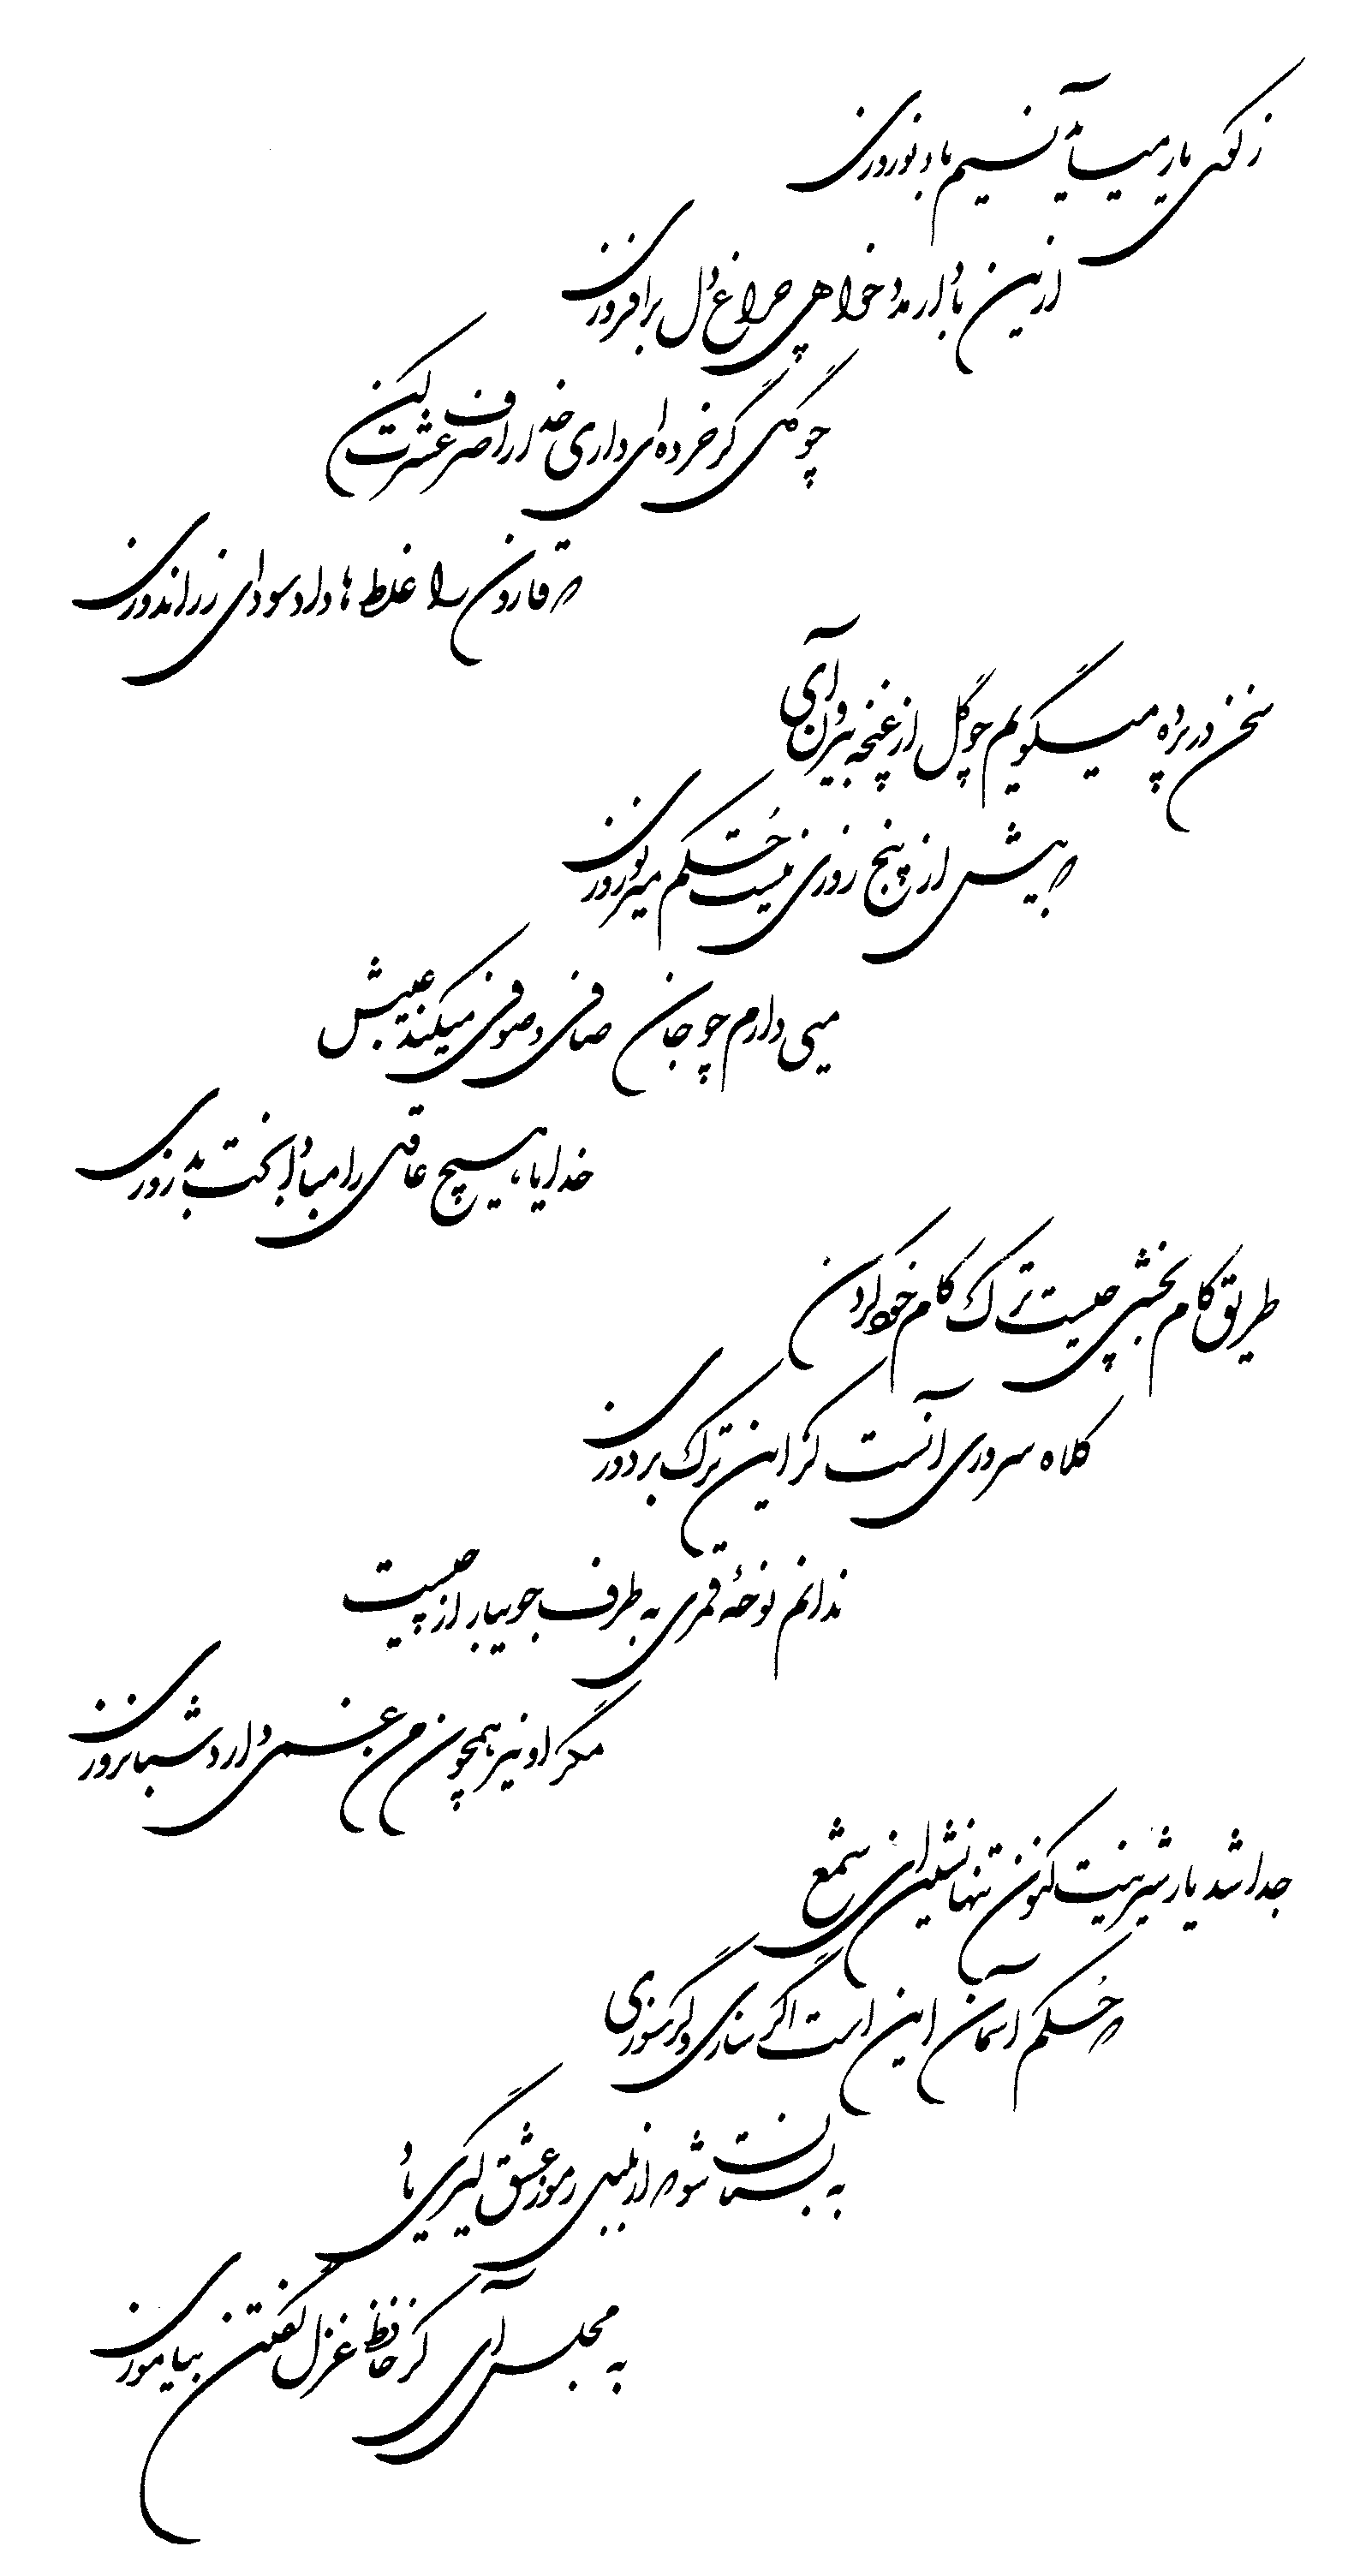
\includegraphics[width=6cm]{hafez.png}\\
\vspace{\fill}
{\LARGE Perzsa négysoros versek}
\end{titlepage}

\thispagestyle{empty}
\begin{center}
  A kötetben szereplő fordítások alapjául szolgáló mű:\\
  \bigskip
  Reza Saberi: A Thousand Years of Persian Rubáiyát.\\
  IBEX (2000)\\
  \bigskip
  A versváltozatok keresésekor nagy segítséget nyújtott\\
  a Ganjoor weboldal is (http://ganjoor.net/).\\
  \bigskip
  Magyar fordítás\ \textcopyright\ Salvi Péter, 2020
\end{center}
\vspace*{\fill}
{\small Ez a könyv a \XeLaTeX\ rendszer segítségével készült, a Bembo stílusú \emph{FBB},
  valamint az \emph{Iran Nastaliq} és \emph{Amiri} betűtípusok felhasználásával.\\
  A címlapon Hâfez egy verse látható egy 1980-as évekből származó újévi üdvözlőlapról.
}



\clearpage
\thispagestyle{plain}
\begin{center}
  \vspace*{\fill}
  {\Large\emph{Szüleimnek}}
  \vspace*{\fill}
\end{center}
\clearpage


\chapter*{Előszó}
\addcontentsline{toc}{chapter}{Előszó}
A perzsa \emph{robâi} négysoros versek az európai ember számára \emph{Omar
Khayyâm} költeményeit jelentik, pedig Perzsiában ez a körülbelül ezer
éves műfaj állandó népszerűségnek örvendett, és minden ismertebb tudós
és költő alkotott benne.

Ebben a kötetben kiválogattam néhány olyan verset, amelyek valami
miatt szerintem különlegesek. Ez lehet egy ügyes szójáték, egy érdekes
gondolat, egy meglepő kép - valami, ami miatt kilép a vers az erősen
kötött forma és a hagyományos témák keretein kívülre.

A \emph{robâi} versek témája három nagy csoportra osztható:

\begin{enumerate}
\item A földi lét gyors elmúlása, a ma élvezete. Gyakori
  szimbólum a föld és az agyag, amibe porhüvelyünk visszatér, illetve
  a bor és a bort töltő \emph{sâqi}.
\item Szerelmes vers a Kedveshez. Mivel a perzsában a személyes névmás
  nemtől független, az esetek nagy részében csak találgathatunk, hogy
  nőkhöz vagy férfiakhoz íródtak, de feltételezhető, hogy sokat írtak
  fiatal fiúkhoz. Itt gyakorta megjelennek híres szerelmespárok, mint
  az őrült \emph{Majnun} és \emph{Layla}, vagy \emph{Farhâd} és
  \emph{Shirin}. Kedvelt szimbólum a bülbül-madár, aki egész éjjel
  énekel hajthatatlan szerelméhez, a rózsához, vagy az éjjeli lepke,
  akit vonz a gyertya lángja, amiben aztán elég.
\item Szúfi vallásos vers. Ez az előző kategóriától nem mindig válik
  el élesen, mert a szúfi gondolkodásmód szerint Isten a Kedves,
  aki iránt való szerelem, és az abban való egyesülés, az Éntől való
  megszabadulás, a földi lét egyetlen értelme. Itt minden szó új
  jelentést kap -- a bor pl.~általában az igazságot, az Istenhez való
  közelséget jelenti, a kocsma a világ stb. A világmindenség titkait
  kendő fedi, ami mögé csak a kiválasztottak nyernek bepillantást.
\end{enumerate}

A fordítások pontosan tartják az eredeti versformát, néhol a pontosság
kárára. Igyekeztem azonban minél kevésbé eltérni az eredetitől, és
megtartani annak legalább szellemét, ha a pontos szavakat nem is
mindig sikerült.

A perzsa nyelv tanulói számára minden versnél szerepel az eredeti
szöveg és annak egy latin betűs átírása is. Mivel a nyelv az utóbbi
ezer évben keveset változott, azt remélem, hogy a fordítás és egy
szótár segítségével az értelmezés nem jelenthet gondot, és így talán
az eredeti vers élvezetét is sikerül hozzáférhetőbbé tennem.

\begin{flushright}
  Salvi Péter, 2020
\end{flushright}


\chapter*{Kiejtés}
\addcontentsline{toc}{chapter}{Kiejtés}
A perzsa nyelvnek különböző változatait beszélik ma Iránban,
Afganisztánban és Tádzsikisztánban, és ezeknek kiejtése
különböző. Noha a dári jobban megtartotta a klasszikus perzsa
magánhangzórendszert, itt mégis inkább a nemzetközileg ismertebb iráni
perzsa kiejtést ismertetem.

A latin betűs átírás a kettőshangzók írásmódjának kivételével
Thackstont\footnote{W.~M.~Thackston: \emph{An Introduction to Persian,
    4th Ed}. Ibex Publishers, 2009.} követi.

A magyartól eltérő kiejtésű betűket és betűkombinációkat a következő
oldalon található táblázat tartalmazza. Ezekhez további megjegyzések:

\begin{itemize}
  \item A \emph{ch}, \emph{k}, \emph{p}, \emph{t} hangok hehezetesek,
    kiejtésükkor több levegőt kell kifújni, mint a magyarban.
  \item A \emph{g} és \emph{k} hangok szótag végén és
    \emph{e}/\emph{i}/\emph{a} magánhangzók előtt palatalizálódnak,
    tehát ilyenkor kiejtésüket egy rövid [j] hang követi.
  \item Az \emph{i} más magánhangzók és \emph{y} előtt [i]-re rövidül.
  \item A \emph{q} hang magánhangzók közt hörgő párizsi [r] hangba
    válthat át.
  \item A két kettőshangzó az \emph{ey} és az \emph{ow}, melyek ejtése
    rendre [éj] és [ou].
\end{itemize}

A hangsúly legtöbb esetben a szó végére kerül; a hangsúlytalan
szuffixumokat kötőjellel jeleztem.

\begin{table}[h]
  \begin{center}
    \smallskip\smallskip
    \begin{tabular}{cl}
      \emph{a} & rövid [á] és [e] közti hang\\
      \emph{â} & [aa]\\
      \emph{ch} & [cs]\\
      \emph{e} & [e] és rövid [é] közti hang\\
      \emph{i} & [í]\\
      \emph{j} & [dzs]\\
      \emph{kh} & hörgő [h] hang\\
      \emph{q} & hátul képzett [g] hang\\
      \emph{s} & [sz]\\
      \emph{sh} & [s]\\
      \emph{u} & [ú]\\
      \emph{y} & [j]\\
      \emph{zh} & [zs]\\
      \emph{`} & torokzárás, elválasztja a szavakat\\
    \end{tabular}
  \end{center}
  \caption{A latin betűs perzsa átírás kiejtése.}
\end{table}


\chapter*{A \emph{robâi} versforma}
\addcontentsline{toc}{chapter}{A \emph{robâi} versforma}
A \emph{robâi} egy nagyon kötött versforma. A rímképlete $AABA$, tehát
a harmadik sor kivételével mindegyik rímel (néhány versben még a
harmadik is). Így tehát tekinthető egy négysoros \emph{qazal}-nak,
mivel annak rímképlete $AABACADA\dots$ (a borítón egy 16 soros
\emph{qazal} látszik).

A rímelés szabálya egyszerű: a sorok végén egy vagy több hangnak
(köztük legalább egy magánhangzónak)
pontosan meg kell egyeznie. Ez az egyezés tartalmazhat teljes szavakat
is (\emph{refrén}), de mindig kell lennie egy olyan részének is, amely
minden sorban különböző jelentésű. Vegyük például \emph{Rashidoddin
Vatvât} egy versét (\pageref{Vatvat}.~o.). A rímelő sorok mind
a \emph{shavam} refrénre végződnek, előtte pedig a \emph{bihush},
\emph{madhush} és \emph{khâmush} szavak alkotják a rímet. Ezek közt a
pontos egyezés csupán két hang, az \emph{-ush}.

Ez a fajta rímelés időnként kicsit idegen a magyar fülnek, ezért a
fordításokban, bár a rímképletet megtartottam, a magyar rímelés
szabályaihoz igazodtam.

A klasszikus perzsa költészet időmértékes. A versek analizálásához
el kell tudnunk dönteni a szótagok hosszát:

\begin{enumerate}[i)]
  \item \emph{Rövid} szótag az, amelyikben rövid magánhangzó van
    (\emph{a}/\emph{e}/\emph{o} vagy rövidült \emph{i}), és ezt nem
    követi mássalhangzó, pl.~\emph{ze}.
  \item \emph{Hosszú} szótag az, amelyik olyan, mint egy rövid szótag, de
    vagy hosszú magánhangzó van benne (a kettőshangzók is hosszúnak
    számítanak), vagy a magánhangzó ugyan rövid, de azt egyetlen mássalhangzó
    követi. Az első típusra példa a \emph{ru} szó, a másodikra a
    \emph{shab}.
  \item \emph{Nyújtott} szótag az, amelyikben vagy egy hosszú magánhangzó
    után következik mássalhangzó, pl.~\emph{yâr}, vagy
    mássalhangzótorlódást tartalmaz, pl.~\emph{dast}, vagy mindkettő,
    pl.~\emph{mâst}. A nyújtott szótag metrikai szempontból hosszú +
    rövid értékű (\metra{\m\b}).
\end{enumerate}

Van ezen kívül még néhány kivételes eset, amelyekről érdemes szót ejteni.
Egyrészt verssor végén minden szótag hosszúnak számít.
Másrészt egy hosszú magánhangzó után magában álló $n$ hangra végződő
szótag nem lesz nyújtott, így pl.~az \emph{ân} szó hosszúnak számít, míg
az \emph{âb} nyújtottnak. Ettől csak rendkívül ritkán térnek el.

Ha egy mássalhangzóra végződő szót magánhangzóval kezdődő követ, akkor
általában ez utóbbi ,,átvállalja'' az előző szótag utolsó
mássalhangzóját (\emph{liaison}), és ennek megfelelően változik a
szótagok hossza is. Így pl.~a \emph{beh agar} \metra{\m\b\m} helyett
\metra{\b\b\m}, és a \emph{kard az} \metra{\m\b\m} helyett
\metra{\m\m} lesz. Időnként a szavakat mégis szétválasztják, ezt
ilyenkor a második szó előtt egy aposztróffal jelöltem, pl.~\emph{beh
'agar}.

Szintén előfordul, hogy a ritmus kedvéért megnyújtják a rövid \emph{e}
és \emph{o} magánhangzókat. Ez különösen gyakran jelentkezik az `és'
jelentésű \emph{-o} szónál, és a perzsa nyelv jellegzetes
struktúra-összekötő \emph{-e} szuffixumánál, valamint az egyesszám
második személyű személyes névmásnál (\emph{to}). E\-ze\-ket a
változásokat makronnal jeleztem (\emph{ē}/\emph{ō}).

A \emph{robâi} ritmusa minden sorban (egymástól függetlenül) kétféle
lehet:
\begin{center}
  {\large\metra{\m\m\mbb\s\m\m\mbb\s\m\m\mbb\s\m\cc}}\\
  vagy\\
  {\large\metra{\m\m\mbb\s\m\b\m\b\s\m\m\mbb\s\m\cc}}
\end{center}

A fordítások is ezt követik, de természetesen a magyar nyelv
szótaghosszai alapján.

\begin{center}
  \pgfornament[anchor=south,width=20mm]{82}
\end{center}

Érdemes megjegyezni, hogy a perzsa metrikák túlnyomó része leírható
egy nagyon logikus rendszerben.\footnote{F.~Thiesen: \emph{A Manual of
    Classical Persian Prosody -- with chapters on Urdu, Karakhanidic
    and Ottoman prosody}. Otto Harrassowitz, Wiesbaden, 1982.}

Jelöljük számokkal az alábbi lábakat:
\begin{center}
  1.~\metra{\b\m\m}\quad 2.~\metra{\b\m\m\m}\quad 3.~\metra{\b\b\m\m}\quad
  4.~\metra{\b\m\b\m\b\b\m\m}\quad 5.~\metra{\m\m\b\b\m\b\m\b}
\end{center}

Ekkor az $i.j.k$ hármas által jelölt ritmust úgy kapjuk meg, hogy az
$i$-edik láb $j$-edik szótagjától kezdve $k$ szótagot veszünk,
folyamatosan ismételve a lábat, pl.:
\begin{center}
4{.}5{.}11 \metra{\b\b\m\m\s\b\m\b\m\s\b\b\m}
\end{center}
Itt a 4.~láb (\metra{\b\m\b\m\b\b\m\m}) 5.~szótagjától, tehát a második felétől kezdve
számolunk le 11 szótagot, a láb utolsó (8.)~szótagja után a láb elejétől folytatva.

Amennyiben a sor végére rövid szótag esne, ez automatikusan hosszú
lesz, pl.:
\begin{center}
4{.}7{.}7 \metra{\m\m\b\m\b\m\m}
\end{center}

Ezekben a mértékekben a két rövid szótagot (\metra{\b\b})
helyettesítheti egy hosszú (\metra{\m}), kivéve a sor legelején, ahol
egy hosszú és egy rövid (\metra{\m\b}) kerülhet a helyére, így a fenti
példa képlete pontosabban:
\begin{center}
4{.}5{.}11 \metra{\mb\b\m\m\s\b\m\b\m\s\mbb\m}
\end{center}

Ez alapján a \emph{robâi} sorok két variánsa megfelel a 3{.}3{.}13
ill.~5{.}1{.}13 képleteknek.

\bigskip

További gyakori konfigurációk:
\begin{framed}
\begin{tabular}{llll}
1{.}1{.}11 & {} & {} & {} \\
2{.}1{.}11 & 2{.}1{.}16 & 2{.}4{.}11 & 2{.}4{.}15 \\
3{.}1{.}15 & 3{.}3{.}14 & {} & {} \\
4{.}5{.}11 & 4{.}7{.}7$^\dagger$ & 4{.}7{.}14 & {} \\
5{.}1{.}10 & {} & {} & {}
\end{tabular}

$^\dagger$ Duplázva, a két félsor közt cezúrával.
\end{framed}

\medskip

Ezek közül kiemelendő a \emph{Királyok könyvé\/}ben is használt eposzi verselés (1{.}1{.}11), illetve
a páronként rímelő sorokból álló \emph{masnavi} költeményekben alkalmazott 2{.}4{.}11 lüktetés (pl.~\emph{A madarak tanácskozása}).


\mainmatter
\pagenumbering{arabic}
\addcontentsline{toc}{chapter}{Versek}
\part*{Versek}
%% -*- bidi-paragraph-direction: left-to-right -*-
\poem{Rudaki}{رودکی}{
جز حادثه هرگز طلبم کس نکند & یک پرسش گرم جز تبم کس نکند\\
ور جان به لب آیدم بجز مردم چشم & یک قطرهٔ آب بر لبم کس نکند
}{
joz hâdese hargez talab-am kas nakonad\\
yek porsesh-e garm joz tab-am kas nakonad\\
v-ar jân be lab âyadam be joz mardom-e cheshm\\
yek qatre-ye âb bar lab-am kas nakonad
}{
Már látogatóba nem jön el más, csak a gond,\\
s nincs más, csak a láz, mely meleg üdvözlést mond.\\
Egy csepp vizet ajkamra nem ad más, csak a szem,\\
lelkem mikor eltávozik, és könnyeket ont.
}{
\emph{Rudaki\/}t (859{--}940) az újperzsa nyelv első
nagy költőjeként tartják számon. Hozzá fűződik
a versek \emph{divân\/}ba rendezése is.
}
\poem{`Onsori}{عنصری}{
گفتم که چرا چو ابر خون بارانم & گفت از پی آن که من گل خندانم\\
گفتم که چرا بی تو چنین پژمانم & گفت از پی آن که تو تنی من جانم
}{
goftam ke cherâ cho abr khun bârânam?\\
goft az pey-e ân ke man gol-ē khandân-am\\
goftam ke cherâ bi to chonin pezhmân-am?\\
goft az pey-e ân ke tō tan-i man jân-am
}{
,,Vért'' -- kérdte -- ,,miért ontok, mint egy felleg?''\\
,,Mert rózsa vagyok'' -- felelt -- ,,virítok s döflek.''\\
,,Mondd akkor: nélküled miért csüggedek én?''\\
,,Mert'' -- mondta -- ,,te test vagy, én azonban lélek.''
}{
\emph{`Onsori} (kb.~961{--}1039) udvari költő,
ódáit az ékesszólás és a formai tökély jellemzi.
Műveinek csak egy töredéke maradt ránk.
}
\poem{Abu Sa'id Abolkheyr}{ابوسعید ابوالخیر}{
جسمم همه اشک گشت و چشمم بگریست & در عشق تو بی‌جسم همی باید زیست\\
از من اثری نماند این عشق ز چیست & چون من همه معشوق شدم عاشق کیست
}{
jesm-am hame ashk gasht o cheshm-am begrist\\
dar `eshq-e to bi-jesm hami bâyad zist\\
az man 'asar-i namânad in `eshq ze chi-st\\
chon man hame ma`shuq shodam `âsheq ki-st
}{
Könnyé vált testem, s elsírtam mindet,\\
test nélkül kell élnie annak, ki szeret.\\
Honnan jön e vágy, mikor nyomom sincs itt már?\\
Eggyé váltunk -- most a Szerelmes ki lehet?
}{
\emph{Abu Sa'id Abolkheyr} (967{--}1049) szúfi gondolkodó.
A mai türkmén határ közelében élt, de híre Spanyolországig eljutott.
Tanítása meghatározó volt a szúfi miszticizmusban,
de ő maga nem írt jelentősebb filozófiai művet.

Jól ismerte Avicennát (\emph{Ebn Sinâ}):
több találkozásukról is írt az önéletrajzában,
és néhány vele váltott levele is fennmaradt.
}
\poem{Qatrân Tabrizi}{قطران تبریزی}{
ای زلف تو از رخان من پرچین‌تر & وز خون دو چشم من رخت رنگین‌تر\\
هر روز تو نیکوتر و من زارترم & هر روز تو دلبرتر و من بی‌دین‌تر
}{
ey zolf-e to az rokhân-e man por-chintar\\
v-az khun-e do cheshm-e man rokh-et rangintar\\
har ruz to nikutar-o man zârtar-am\\
har ruz to delbartar-o man bi-dintar
}{
Arcomnál fodrosabb a dús hajfonatod,\\
vérző szemeimnél pirosabb még arcod.\\
Szebb vagy minden nap, s nyomorultabb vagyok én,\\
és egyre hitetlenebb, ha látom alakod.
}{
\emph{Qatrân Tabrizi} (1009{--}1072) azeri költő. Elsősorban ódáiról és
dicshimnuszairól híres, melyeket kb.~30 különböző mecénáshoz írt.
}
\poem{`Omar Khayyâm}{عمر خیام}{
آن قصر که با چرخ همی زد پهلو & بر درگه آن شهان نهادندی رو\\
دیدیم که بر کنگره‌اش فاخته‌ای & بنشسته همی گفت که کوکوکوکو
}{
Ân qasr ke bâ charkh hami zad pahlu\\
Bar dargah-e ân shahân nehâdandi ru\\
Didim ke bar kongere-ash fâkhte-i\\
Benshaste hami goft ke kukukuku
}{
Ez volt az az Éggel versengő palota,\\
sok sah kapujában hajlongott valaha.\\
Most egy madarat láttam a csipkés bástyán --\\
ott ült s így szólt: ,,Kakukk! Kakukk! Minden oda!''
}{
\emph{`Omar Khayyâm} (1048{--}1131) matematikus, csillagász és költő.
Versei a XIX.~század második felében Európa-szerte ismertek lettek Edward
FitzGerald átköltésein keresztül.
}
\poemnotoc{`Omar Khayyâm}{عمر خیام}{
از آمدن بهار و از رفتن دی & اوراق وجود ما همی گردد طی\\
می خور مخور اندوه که فرمود حکیم & غمهای جهان چو زهر و تریاقش می
}{
az 'âmadan-ē bahâr-o az raftan-e dey\\
owrâq-e vojud-e mâ hami gardad tey\\
mey khor makhor anduh ke farmud hakim\\
qamhâ-ye jahân cho zahr-o teryâq-esh mey
}{
Már elmegy a tél, jő a tavasz, rajta a sor,\\
apránként így lapozza létünket a Kor.\\
Koccints, ne szomorkodj, hisz' az orvos mondta:\\
méreg minden gond, s rá ellenszer a bor.
}{
Tudományos munkáiban többek közt geometriai megoldást adott
kúpszeletek metszésére, és megalkotta a \emph{Jalâli} naptárat,
melynek változatai ma is használatban vannak Iránban és
Afganisztánban.  Foglalkozott a zenei skálák matematikai
rendszerezésével is.
}
\poem{Abolfazl Rashidoddin Meybodi}{ابو‌الفضل رشیدالدین میبدی}{
ز اول که مرا عشق نگـارم نو بود & همسایه به شب ز نالهٔ من نغنود\\
کم گشت کنون ناله که عشقم بفزود & آتش چو همه گرفت کم گردد دود
}{
z-avval ke ma-râ `eshq-e negâr-am now bud\\
  hamsâye be shab ze nâle-yē man naqonud\\
kam gasht konun nâle ke `eshq-am bofzud\\
  âtesh cho hamē gereft kam gardad dud
}{
Nem hagytam a szomszédnak régen pihenést,\\
úgy sóhajtoztam este, vágyván ölelést.\\
Csökkentek a sóhajok, szerelmem hogy nőtt:\\
nem füstöl a tűz, ha lángja mindent felemészt.
}{
\emph{Abolfazl Rashidoddin Meybodi} (XII.~sz.~eleje)
szunnita szúfi tudós. Életéről keveset tudni,
de fennmaradt fő műve, egy monumentális Korán-kommentár.
}
\poem{Mahsati Ganjavi}{مهستی گنجوی}{
چشمم چو به چشم خویش چشم تو بدید & بی چشم تو خواب چشمم از چشم پرید\\
ای چشم همه چشم به چشمت روشن & چون چشم تو چشم من دگر چشم ندید
}{
cheshm-am cho be cheshm-e khish cheshm-ē to bedid\\
bi cheshm-e to khâb-e cheshm-am az cheshm parid\\
ey cheshm hamē cheshm be cheshm-et rowshan\\
chon cheshm-e to cheshm-e man degar cheshm nadid
}{
Láttam szemedet saját szememmel, s emiatt\\
estére szememből álmom messze szaladt.\\
Ó szem, mire minden szemnek fénye vetül,\\
nincs más szempár sehol, szemem min megakad.
}{
\emph{Mahsati} ,,Hold-asszony'' (1089{--}1175?) azerbajdzsáni költőnő.
Szókimondó versei és szabadelvű élete miatt sok üldöztetésben volt része.
}
\poem{`Eynolqozât Hamadâni}{عین‌القضات همدانی}{
ناگه ز درم درآمد آن دلبر مست & جام می لعل نوش کرد و بنشست\\
از دیدن و از گرفتن زلف چو شست & رویم همه چشم گشت و چشمم همه دست
}{
nâgah ze dar-am dar-âmad ân delbar-e mast\\
jâm-ē mey-e la`l nush kard-ō benshast\\
az didan-o az gereftan-ē zolf cho shast\\
ruy-am hame cheshm gasht-o cheshm-am hame dast
}{
Ő hirtelen ajtóm küszöbén átlépett\\
s bort íva magához húzott egy széket.\\
Gyűrűző fürtjét hogy lássam s fogjam,\\
arcom csupa szem, szemem pedig mind kéz lett.
}{
\emph{`Eynolqozât} ,,bírók gyöngye'' \emph{Hamadâni} (1098{--}1131) jogász,
szúfi filozófus, költő és matematikus, \emph{`Omar Khayyâm} tanítványa.
Eretnekségért 33 éves korában kivégezték.
}
\poem{Rashidoddin Vatvât}{رشید‌الدین وطواط}{\label{Vatvat}
بویت شنوم ز باد بی‌هوش شوم & نامت شنوم ز خلق مدهوش شوم\\
اول سخنم توئی چو در حرف آیم & واندیشهٔ من توئی چو خاموش شوم
}{
buy-et shenavam ze bâd bihush shavam\\
nâm-et shenavam ze khalq madhush shavam\\
avval sokhan-am to-i cho dar harf âyam\\
v-andishe-ye man to-i cho khâmush shavam
}{
Szél illatodat ha hozza, mámorba esem;\\
mástól nevedet ha hallom, elvesztem eszem.\\
Szólok -- s első szavam te vagy; nem szólok --\\
s csak téged idéz némán emlékezetem.
}{
\emph{Rashidoddin Vatvât} (1114?{--}1182) szunnita
költő a mai Afganisztán területéről.
A Hvárezmi Birodalomban udvari költőként szolgált.
}
\poem{Ruzbehân Baqli}{روزبهان بقلی}{
دی آینهٔ خویش به صیقل دادم & روشن کردم به پیش خود بنهادم\\
در آینه عیب خویش چندان دیدم & کز عیب کسان هیچ نیامد یادم
}{
di âyene-yē khish be seyqal dâdam\\
rowshan kardam be pish-e khod benhâdam\\
dar 'âyene `eyb-e khish chandân didam\\
k-az `eyb-e kasân hich nayâmad yâd-am
}{
Tegnap lecsiszoltam ezt a tükröt szépen,\\
míg fényes nem lett, s ahogy állt egy széken,\\
rápillantván annyi hibámat láttam,\\
hogy nem jut eszembe most a másé éppen.
}{
\emph{Ruzbehân Baqli} (1128{--}1209) szúfi misztikus filozófus és költő.
Leghíresebb művét, egy látomásokkal teli napló-önéletrajzot,
\emph{A titkok felfedésé\/}t, arabul írta. (1943-ban Khomeyni ugyanezen
a címen publikálta először politikai nézeteit.)
}
\poem{Attâr Neyshâburi}{عطار نیشابوری}{
بازی بودم پریده از عالم راز & تا بو که برم ز شیب صیدی به فراز\\
اینجا چه نیافتم کسی‌را دمساز & زان در که بیآمدم برون رفتم باز
}{
bâz-i budam paride az `âlam-e râz\\
tâ bu ke baram ze shib seyd-i be farâz\\
injâ che nayâftam kas-i-râ damsâz\\
z-ân dar ke biâmadam berun raftam bâz
}{
Titkok völgyéből, mint egy héjamadár,\\
zsákmányommal magasba felszálltam már;\\
ám most a kapun, melyen bejöttem, kimegyek,\\
mert nem leltem barátot, itt senki se vár.
}{
\emph{Attâr} ,,gyógyfüves'' \emph{Neyshâburi} (1145{--}1221) költő,
szúfi gondolkodó és hagiográfus. Gyógyszerészként dolgozott, majd
üzletét otthagyva utazni kezdett, eljutott Mekkába és Indiába is.
Munkássága nagy hatással volt \emph{Rumi\/} költészetére.
(Ezt a verset más forrásokban \emph{Rumi\/}nak tulajdonítják.)\\
Fő művét, \emph{A madarak tanácskozásá\/}t, magyarra is lefordították.
}
\poem{Majdoddin Baqdâdi}{مجدالدین بغدادی}{
شمع است رخ خوب تو پروانه منم & دل خویش غم تو است و بیگانه منم\\
زنجیر سر زلف که بر گردن تست & در گردن من فکن که دیوانه منم
}{
sham`-ast rokh-ē khub-e to parvâne man-am\\
del khish-e qam-ē to-ast-o bigâne man-am\\
zanjir-e sar-ē zolf ke bar gardan-e to-st\\
dar gardan-e man fakan ke divâne man-am
}{
Szép arcod gyertyaláng, e fényhez repked\\
szívem, mint egy moly, idegenként, s szenved;\\
dobd hát a nyakadról hajfürtöd láncát\\
béklyóként rám, ki érted őrülten eped.
}{
\emph{Majdoddin Baqdâdi} (1158{--}1211) orvos,
a \emph{kobrawi} szúfi rend alapítójának,
\emph{Najmoddin Kobrá\/}nak legkedvesebb tanítványa,
és feltehetőleg a híres költő, \emph{Attâr} mestere.
Elsősorban teológiai tárgyú műveket írt, perzsául és arabul is,
leghíresebb közülük a \emph{Resâle dar safar} (Levél az utazásról).
A sah anyjával való kapcsolata miatt kivégezték:
beledobták az \emph{Âmudaryâ} (görög \emph{Oxos}) folyóba.
}
\poem{Kamâloddin Esmâ`il}{کمال‌الدین اسماعیل}{
هر شب ز غمت تو ای نگارین یارم & وز مهر رخ چو ماهت ای دلدارم\\
تا وقت سحر به ماه در می‌نگرم & وز دیده ستارگان فرو می‌بارم
}{
har shab ze qam-et to ey negârin yâr-am\\
v-az mehr-ē rokh cho mâh-et ey deldâr-am\\
tâ vaqt-e sahar be mâh dar-minegaram\\
v-az dide setâregân foru mibâram
}{
Szép kedvesem, arra vágyom, éljél te velem:\\
hold-arcod az ok, hogy éjjel én rendszeresen\\
hajnalhasadásig csak a Holdat nézem,\\
és csillagokat záporozik tőle szemem.
}{
\emph{Kamâloddin Esmâ`il} (1173{--}1237) költő,
elsősorban ódáiról híres.
}
\poem{Rumi}{رومی}{\label{Rumi}
خورشید و ستارگان و بدر ما اوست & بستان و سرای و صحن و صدر ما اوست\\
هم قبله و هم روزه و صبر ما اوست & عید و رمضان و شب قدر ما اوست
}{
khorshid-o setâregân-o badr-ē mâ u-st\\
bostân-o sarây-o sahn-o sadr-ē mâ u-st\\
ham qeble-o ham ruze-o sabr-ē mâ u-st\\
`id-ō ramazân-ō shab-e qadr-ē mâ u-st
}{
Nap, csillagok és Hold, tündöklő -- ez is Ő.\\
Udvar, kert, otthon, s asztalfő -- ez is Ő.\\
Böjt és türelem, kibla, a szent kő -- ez is Ő.\\
Kadr-éj Ramadánkor, ó, ha eljő -- ez is Ő.
}{
\emph{Rumi\/} (1207{--}1273) szúfi teológus és költő. Versei
meghatározó hatással voltak nemcsak a perzsa,
hanem a környező népek irodalmára nézve is.
Műveit számos nyelvre lefordították; népszerűségét mutatja, hogy
gyakran csak úgy hivatkoznak rá, hogy \emph{Mowlânâ} ,,u\-runk''.
Költeményeiben írt törökül, arabul és görögül is.
}
\poem{Sa`di}{سعدی}{
آن یار که عهد دوستداری بشکست & می‌رفت و منش گرفته دامان در دست\\
می‌گفت دگر باره به خوابم بینی & پنداشت که بعد از آن مرا خوابی هست
}{
ân yâr ke `ahd-e dustdâri beshekast\\
miraft-o man-esh gerefte dâmân dar dast\\
migoft degar bâre be khâb-am bini\\
pendâsht ke ba`d az ân ma-râ khâb-i hast
}{
Egy nap, mikor esküvéseit szegve a párom\\
elment, szólt, hogy nem érdemes rá várnom:\\
,,Álmodban fogsz csak engem újból látni!''\\
Csak nem hiszi, hogy szememre jön még álom?
}{
\emph{Sa`di} (1210{--}1291) író, költő.
Prózai művei, mint a \emph{Gyümölcsöskert} és a \emph{Rózsakert}
az egyszerű, de elegáns, kifinomult stílus mintapéldái.
Fiatalkorában sokat utazott, harcolt a kereszteslovagok ellen,
és hét évet fogságban töltött Akkóban.
}
\poemnotoc{Sa`di}{سعدی}{
آنان که پری‌روی و شکرگفتارند & حیفست که روی خوب پنهان دارند\\
فی‌الجمله نقاب نیز بی‌فایده نیست & تا زشت بپوشند و نکو بگزارند
}{
ânân ke pari-ruy-o shekar-goftâr-and\\
heyf-ast ke ruy-e khub penhân dârand\\
feljomle neqâb niz bi-fâyede nist\\
tâ zesht bepushand-o neku bogzârand
}{
Mily kár, hogy a sok tündér utcára ha lép,\\
arcát mind elrejti, s nem látja a nép.\\
Van haszna a fátyolnak azért mégis tán:\\
hogy felvegye az, ki csúnya, s eldobja, ki szép.
}{
}
\poem{`Alâ'oddowle Semnâni}{علاءالدوله سمنانی}{
وقت سحری در‌آمد آن مهرویم & در گوش دلم گفت که ای دلجویم\\
تو هیچ مباش تا همه من باشم & تو هیچ مگوی تا همه من گویم
}{
vaqt-ē sahar-i dar-âmad ân mahru-yam\\
dar gush-e del-am goft ke ey delju-yam\\
tō hich mabâsh tâ hamē man bâsham\\
tō hich maguy tâ hamē man guyam
}{
Hold-arcú kedvesem szobámban jár-kel,\\
szívemhez szól, fülembe súg, így ráz fel:\\
,,Légy semmi, hogy én váljak a mindenséggé;\\
s hogy mindent elmondjak, hallgassál el.''
}{
\emph{`Alâ'oddowle Semnâni} (1261{--}1336) szúfi filozófus
a \emph{kobraviye} rendből.
}
\poemnotoc{`Alâ'oddowle Semnâni}{علاءالدوله سمنانی}{
صد خانه اگر به طاعت آباد کنی & به زان نبود که خاطری شاد کنی\\
گر بنده کنی ز لطف آزادی‌را & بهتر که هزار بنده آزاد کنی
}{
sad khâne agar be tâ`at âbâd koni\\
beh z-ân nabovad ke khâter-i shâd koni\\
gar bande koni ze lotf 'âzad-i-râ\\
behtar ke hazâr bande âzâd koni
}{
Építhetsz szentélyt, száz fajtát-formát:\\
egy kedves szócska többet ér majd odaát.\\
Jobb egy szabad embert leigáznod keggyel,\\
mint felszabadítanod ezer rabszolgát.
}{
}
\poem{Hâfez}{حافظ}{
چون جامه ز تن برکشد آن مشکین خال & ماهی که نظیر خود ندارد به کمال\\
در سینه ز نازکی دلش بتوان دید & مانندهٔ سنگ خاره در آب زلال  
}{
chon jâme ze tan bar-kashad ân moshkin khâl\\
mâh-i ke nazir-e khod nadârad be kamâl\\
dar sine ze nâzoki del-esh betvân did\\
mânande-ye sang-e khâre dar 'âb-e zolâl
}{
Mint páratlan szépségű hold, olyan ő,\\
arcán anyajeggyel, ha levetkőzik e nő.\\
Mellén, bizony oly törékeny, átsejlik a szív,\\
mint kristálytiszta vízen egy gránitkő.
}{
\emph{Hâfez} (1315{--}1390) költészetét a perzsa irodalom csúcsának tekintik;
versgyűjteménye (a Korán mellett) gyakori eleme az újévi dekorációnak.
Szerelmes versei értelmezhetőek szó szerint és szimbolikusan is,
ami nem kevés vitára adott okot.
\emph{Divân\/}jából -- ahogy régen Vergilius műveiből -- ma is gyakran jósolnak
a perzsa nyelvterületeken.
}
\poem{Shâh Ne`matollâh Vali}{شاه نعمت‌الله ولی}{
صبح و سحر و بلبل و گلزار یکیست & معشوقه و عشق و عاشق و یار یکیست\\
هر چند درون خانه را می‌نگرم & خود دایره و نقطه و پرگار یکیست
}{
sobh-ō sahar-ō bolbol-o golzâr yek-i-st\\
ma`shuqe-o `eshq-o `âsheq-ō yâr yek-i-st\\
har chand darun-e khâne-râ minegaram\\
khod dâyere-ō noqte-o pargâr yek-i-st
}{
Éj, hajnal, bülbül és virágtő -- mind egy;\\
vágy és szerelem, barát-barátnő -- mind egy.\\
Bárhányszor nézem én a Házat s mit rejt:\\
Én és a Kör és a Pont s a Körző -- mind egy.
}{
\emph{Shâh Ne`matollâh Vali} (1330{--}1431?) szúfi szent,
a \emph{ne`matollâhi} rend alapítója. Sírja zarándokhely \emph{Mâhân\/}ban.
A versben a Pont (vagy ,,a Kör pontja'') Mohamedre utal; a Kör a világ, a Körző a Teremtő.
}
\poem{Abolvafâ Khârazmi}{ابو‌الوفا خوارزمی}{
بر عقل چو کشف پرده‌ها بود محال & عقل از پس پرده کرد از عشق سؤال\\
تا هست رونده هستی اوست حجاب & ور نیست شود که بهره یابد ز وصال
}{
bar `aql cho kashf-e pardehâ bud mahâl\\
`aql az pas-e parde kard 'az `eshq soâl\\
tâ hast ravande hasti-yē u-st hejâb\\
v-ar nist shavad ke bahre yâbad ze vasâl
}{
Nem képes Ész a leplen átlátni, s ezért\\
függöny mögül ő útmutatást Vágytól kért:\\
,,Falként fedi el léte a vándort, de ha ő\\
nincsen, a haszon kié, ha céljához elért?''
}{
\emph{Abolvafâ Khârazmi} (?{--}1431) szúfi tanító, költő.
}
\poemnotoc{Abolvafâ Khârazmi}{ابو‌الوفا خوارزمی}{
آمد بر من خیال او نیم شبان & گفتم که نثار پای تست این دل و جان\\
گفتا چه دل و چه جان ترا ملک کجاست & آسان باشد سخاوت از مال کسان
}{
âmad bar man khayâl-e u nim-e shabân\\
goftam ke nesâr-e pâ-ye to-st in del-o jân\\
goftâ che del-ō che jân to-râ melk kojâ-st\\
âsân bâshad sakhâvat az mâl-e kasân
}{
Álomkép jött el éjjel, ébenfa-hajú,\\
mondtam, hogy ,,E szívet s lelket vidd, te fiú!''\\
Szólt: ,,Mely szív és lélek? Hol van, mi tiéd?\\
Könnyen vagy a másokéval ily nagyvonalú.''
}{
}
\poem{Jâmi}{جامی}{
دیدار تو ای یار پسندیدهٔ من & حیف است بدین دیدهٔ غمدیدهٔ من\\
در دیدهٔ من نشین و بغشای نقاب & خود بین رخ خویش لیکن از دیدهٔ من
}{
didâr-e to ey yâr-e pasandide-ye man\\
heyf-ast bed-in dide-ye qamdide-ye man\\
dar dide-ye man neshin va-bogshây neqâb\\
khod bin rokh-e khish liken az dide-ye man
}{
Szépséged, kedves, kivetett rám sarcot,\\
csüggedt szemeim már nem akarnak harcot.\\
Ülj hát a szemembe, vesd le kendőd, s te magad\\
bámuld a szemem lencséjén át arcod.
}{
\emph{Jâmi\/}t (1414{--}1492) a középkori perzsa irodalom utolsó nagy költőjeként tartják számon.
Verses és prózai művei mellett számos filozófiai, teológiai és nyelvészeti tárgyú könyvet is írt.
}
\poem{Feyzi}{فیضی}{
آن نیست که ما ارض و سما نشناسیم & تیر قدر و راز قضا نشناسیم\\
این هژده هزار عالم و هر چه در اوست & نشناخته به اگر ترا نشناسیم
}{
ân nist ke mâ arz-o samâ nashnâsim\\
tir-ē qadr-ō râz-e qazâ nashnâsim\\
in hezhde-hazâr `âlam-ō har che dar u-st\\
nashnâkhte beh 'agar to-râ nashnâsim
}{
Számomra a Föld, s az Ég a Földnek peremén,\\
titkot nem rejt, tudom, mi bűn és mi erény.\\
Inkább sokezer világot, és benne mi van,\\
mindent feledek, de téged ismerjelek én.
}{
\emph{Feyzi} (1547{--}1595) indiai költő, Akbar történetírójának bátyja.
Ő fordította le perzsára a híres XII.~századi szanszkrit matematikai művet,
a Līlāvatī-t. Arabul is írt.
}
\poem{Sheykh Bahâi}{شیخ بهای}{
در میکده دوش زاهدی دیدم مست & تسبـیح به گردن و صراحی در دست\\
گفتم ز چه در میکده جا کردی گفت & از میکده هم به سوی حق راهی هست
}{
dar meykade dush zâhed-i didam mast\\
tasbih be gardan-ō sorâhi dar dast\\
goftam ze che dar meykade jâ kardi goft\\
az meykade ham be su-ye haq râh-i hast
}{
Kocsmában a pultra részeg aszkéta borult,\\
és ujjai közt rózsafüzérhez kupa bújt.\\
Megkérdeztem: ,,Te mit csinálsz itt?'', s így szólt:\\
,,Istenhez még kocsmából is vezet út.''
}{
\emph{Sheykh Bahâi} (1547{--}1621) arab származású filozófus, építész, matematikus és csillagász,
az \emph{esfahân\/}i filozófiai iskola alapítója.
}
\poem{Sarmad Kâshâni}{سرمد کاشانی}{
راضی دل دیوانه به تقدیر نشد & فارغ ز خیال فکر و تدبیر نشد\\
ایام شباب رفت و باقیست هوس & ما پیر شدیم و آرزو پیر نشد
}{
râzi del-e divâne be taqdir nashod\\
fâreq ze khayâl-e fekr-o tadbir nashod\\
ayyâm-e shabâb raft-o bâqi-st havas\\
mâ pir shodim-o ârzu pir nashod
}{
Ellenzi a szívem mit a sors néki utal,\\
s tervez: várják még nők és étel-ital.\\
Ifjúkorom elszállt; mi maradt, az csak a vágy.\\
Vén lettem, a szenvedély viszont még fiatal.
}{
\emph{Sarmad Kâshâni} (1590{--}1661) örmény zsidó születésű indiai költő.
Készített egy perzsa Tóra-fordítást is, de később kiábrándult a vallásokból,
és -- egy francia utazó leírása szerint -- \emph{faqir\/}ként, meztelenül,
hosszú hajjal és körmökkel járta Delhi utcáit.
}
\poem{Abdolqâder Bidel}{عبدالقادر بیدل}{
عالم غرض‌آلود جنون من و ماست & اینجا عشق هوس نیالوده کجاست\\
فرهادی و مجنونی اگر می‌شنوی & خود این همه نیست حرف و صوت شعراست
}{
`âlam qaraz-âlud-e jonun-ē man-o mâ-st\\
injâ `eshq-ē havas-nayâlude kojâ-st\\
Farhâd-i-o Majnun-i agar mishenavi\\
khod 'in hame nist harf-o sowt-ē sho`arâ-st
}{
Oly mocskos az Én őrületétől a világ!\\
Hol van szerelem, mit nem szennyez be a vágy?\\
Farhádról vagy Madzsnúnról hallasz tán?\\
Csak költők hangja az, üres líraiság.
}{
\emph{Abdolqâder Bidel} (1642{--}1720) török származású indiai szúfi szent, költő;
\emph{Bidel Dehlavi} ,,delhii Bidel'' néven is ismert.
Tizenhat verseskötetében több, mint 140 ezer vers található.
Egyedi stílusa meghatározó volt az indiai iskola költészetében,
és többek közt nagy hatással volt a legnagyobb urdú költőkre,
\emph{Ghālib\/}ra és \emph{Iqbāl\/}ra is.
}
\poem{Moshtâq Esfahâni}{مشتاق اصفهانی}{
غم بی‌حد و درد بی‌شمار و من فرد & یا رب چه کنم که صبر نتوانم کرد\\
یا درد به اندازهٔ طاقت بفرست & یا حوصله‌ای بده به اندازهٔ درد
}{
qam bi-had-o dard bi-shomâr-ō man fard\\
yâ-rab che konam ke sabr natvânam kard\\
yâ dard be andâze-ye tâqat beferest\\
yâ howsele-i bedeh be andâze-ye dard
}{
Tengernyi a gond, a kín temérdek, s én egy!\\
Mondd, mit tegyek, ó, Uram? A tűrés nem megy!\\
Küldj annyit a kínból, mit erőm még elbír,\\
vagy kínhoz mérten adj türelmet -- mindegy!
}{
\emph{Moshtâq Esfahâni} (1690{--}1758) költő az Afsárida-dinasztia
kezdeti időszakából; a perzsa irodalmi
reneszánsz (\emph{bâzgasht-e adabi}), azon belül is
az \emph{esfahân\/}i stílus egyik korai képviselője.
}
\poem{Malekoshshoarâ Bahâr}{ملک‌الشعراء بهار}{
زاقی می‌گفت اگر بمیرد شهباز & من جای کنم به دست شاهان از ناز\\
بلبل بشنید و گفت کای بندهٔ آز & رو لاف مزن با وزغ و موش بساز
}{
zâqi migoft agar bemirad shahbâz\\
man jây konam be dast-e shâhân az nâz\\
bolbol beshenid o goft k-ey bande-ye âz\\
row lâf mazan bâ vazq-ō mush besâz
}{
Azt mondta a szarka: ,,Hogyha elhull a fehér\\
sólyom, karjára engem ültet a vezér.''\\
Hallotta a bülbül: ,,Ó, mohóság rabja,\\
mit hencegsz?'' -- szólt -- ,,Vár a varangy és az egér!''
}{
\emph{Malekoshshoarâ} ,,költők királya'' \emph{Bahâr} (1886{--}1951), valódi nevén
\emph{Mohammadtaqi Bahâr} iráni költő, politikus,
újságíró és történész. A Tehrán Egyetemen irodalmat tanított, és egy irodalmi folyóiratot
is létesített.
Költeményei hagyományos stílusúak, és gyakran
hazafias hangvételűek.
}
\poemnotoc{Malekoshshoarâ Bahâr}{ملک‌الشعراء بهار}{
برخیز که خود را ز غم آزاده کنیم & تا کی طلب روزی ننهاده کنیم\\
آخر که گل ما به سبو خواهد رفت & کن فکر سبوئی که پر از باده کنیم
}{
bar-khiz ke khod-râ ze qam âzâde konim\\
tâ key talab-ē ruzi-ye nanhâde konim\\
âkhar ke gel-ē mâ be sabu khâhad raft\\
kon fekr-e sabu-'i ke por az bâde konim
}{
Kelj fel, hogy a gondtól szabadítsuk szívünk!\\
Íratlan sorsot még meddig keresünk?\\
Korsó lesz majd porhüvelyünkből úgyis,\\
gondolj a köcsögre, melybe bort töltöttünk!
}{
Ez a vers \emph{Hâfez} egy \emph{qazal\/}jának
parafrázisa, melynek első pár sora:
\begin{Verse}
\emph{beshnow in nokte ke khod-râ ze qam âzâde koni\\
khun khori gar talab-ē ruzi-ye nanhâde koni\\
âkherol'amr gel-ē kuze garân khâhi shod\\
hâliyâ fekr-e sabu kon ke por az bâde koni}
\end{Verse}
}
\poem{Saqir Esfahâni}{صغیر اصفهانی}{
ای ساقی ماه‌وش در این ماه صیام & ده باده که روزه بهر من گشت حرام\\
افطار کنم که دیده ز ابرو و رخت & هم شـکل هلال دید و هم ماه تمام
}{
ey sâqi-ye mâh-vash dar in mâh-e siyâm\\
deh bâde ke ruze bahr-e man gasht harâm\\
eftâr konam ke dide z-abru va-rokh-et\\
ham shakl-e helâl did-o ham mâh-e tamâm
}{
Ó, hold-arcú pohárnokom, jöjj, tölts bort!\\
Bár még Ramadán van, de a böjt nem javasolt,\\
mert orcád és szemöldököd formáján\\
már felragyogott nekem a fél- és telihold.
}{
\emph{Mohammad Hoseyn Saqir Esfahâni} (1894{--}1970) iráni költő.
Különösen misztikus verseiről híres,
a próféta családjának (\emph{ahlol-beyt}) költőjeként tartják számon.
}
\poem{Abolqâsem Hâlat}{ابوالقاسم حالت}{
حیوان درنده‌ای که خونخوار بود & بهتر ز امیری که ستمـکار بود\\
کز آن گاهی به جسم آسیب رسد & وز این همه گاه جان در آزار بود
}{
heyvân-e darande-i ke khunkhâr bovad\\
behtar ze amir-i ke setamkâr bovad\\
k-az 'ân gâhi be jesm 'âsib resad\\
v-az 'in hame gâh jân dar âzâr bovad
}{
Egy vérszomjas vadállat is kellemesebb,\\
mint egy zsarnok, bár legyen ádáz véreb.\\
Mert míg az egyiktől olykor szenved a test,\\
állandó lelki kín a másik, nyílt seb.
}{
\emph{Abolqâsem Hâlat} (1913{--}1992) iráni író, költő;
az 1979-ben alakult Iráni Iszlám Köztársaság első himnuszának szövegírója.
Elsősorban szatíráíról híres.

Ez a vers érdekes párhuzamba állítható a kínai Szertartások könyvének
egy jelenetével, melyben Konfuciusz találkozik egy asz-szonnyal,
aki a zsarnoki uralom elől a tigrisekkel teli erdőbe menekült
(\emph{Lǐ jì: Tán gōng xià 193}).
}
\poem{Javâd Nurbakhsh}{جواد نوربخش}{
بی عشق اگرچه زنده‌ای مرداری & بی عشق اگر عزیز باشی خواری\\
بی عشق اگر شهنشهی مسکینی & با عشق اگرچه عاجزی سرداری
}{
bi `eshq 'agarche zende-i mordâr-i\\
bi `eshq 'agar `aziz bâshi khâr-i\\
bi `eshq 'agar shahanshah-i meskin-i\\
bâ `eshq 'agarche `âjez-i sardâr-i
}{
Vágy nélkül az élő is holt, mint mi kimúlt,\\
vágy nélkül nincsen, ki erős -- mind nyomorult.\\
Vágy nélkül bármi nagy király is koldus:\\
vággyal kap a béna is parancsnok-koszorút.
}{
\emph{Javâd Nurbakhsh} (1926{--}2008) 1953-tól haláláig a \emph{ne'matollâhi}
szúfi rend feje (\emph{pir}), pszichiáter. Orvosi tanulmányait a Sorbonne-on végezte;
az 1979-es forradalom után először Amerikába, majd Angliába emigrált. Számos könyvet írt
a szúfi filozófiáról -- többek közt egy 16-kötetes enciklopédiát a szúfi szimbolizmusról --,
és kiadott egy 30-kötetes pszichiátriai kézikönyvet is.
}
\poem{Mansur Owji}{منصور اوجی}{
ناگاه شبی ز خواب بیدار شدیم & آیـینهٔ راز و رمز اسرار شدیم\\
با بانگ انا الحقی که بر خاک زدیم & منصور شدیم و باز بر دار شدیم
}{
nâgâh shab-i ze khâb bidâr shodim\\
âyine-ye râz-o ramz-e asrâr shodim\\
bâ bâng-e ana-l-haq-i ke bar khâk zadim\\
mansur shodim-o bâz bar dâr shodim
}{
Álmomból felriadva én lettem a Szó:\\
rejtélyek tükre, kulcs, a Titkot kinyitó.\\
,,Isten vagyok én!'' -- szóltam a Földhöz, amitől\\
\emph{Mansur\/}rá váltam és megint vár a bitó.
}{
\emph{Mansur Owji} (1937{--}) iráni költő. A vers egy másik \emph{Mansur\/}ra utal:
\emph{Mansur-e Hallâj} (858{--}922) szúfi misztikus. Híres mondása \emph{'ana l-\d{h}aqq}
,,én vagyok az Igazság/Isten'' (arab), ami miatt halálra ítélték
(bár valószínűleg itt az Istennel való teljes egyesülésre utalt).
}
\poem{Seyyed Mohammad Beheshti}{سید محمد بهشتی}{
دیریست کنار چشمه چشمم نگران & ناگاه مگر ببیـنمت چون دگران\\
پوشی رخ و گویی که گنهکـاری تو & بخشنده توئی گناه خونین جگران
}{
dir-i-st kenâr-e cheshme cheshm-am negarân\\
nâgâh magar bebinam-et chon degarân\\
pushi rokh-o gui ke gonahkâr-i tō\\
bakhshande to-i gonâh-e khunin jegarân
}{
Régóta figyel már a szemem egy patakot,\\
hogy mint mások, megláthatnám alakod.\\
Elrejted az arcod, s bűnösnek nevezel;\\
vérző szívek feloldozását te adod.
}{
\emph{Seyyed Mohammad Beheshti} (1951{--}) iráni építész.
Fontos szerepe volt
a Fajr nemzetközi filmfesztivál, a Farabi filmművészeti alapítvány
és a Turisztikai és Kulturális Örökség Kutatóintézet megalapításában,
illetve az iráni építészeti enciklopédia készítésében.
Számos egyetemen tart előadásokat iráni kultúrtörténetről.
}


\tableofcontents

\end{document}

